\begin{circuitikz}[scale=0.8, transform shape]
            \ctikzset{tripoles/en amp/input height=-0.45}
            \draw (0,0) node[en amp](E){};
            \draw (E.out) node[circ]{} node[right]{$U_A$};
            \draw (E.-) -- ++(0, -1.3) node[circ] {} to[R, l=$R_2$] ++(2.38,0) -- ++(0,1.8);
            \draw (E.-) -- ++(0, -1.3) node[circ] {} to[R, l_=$R_1$] ++(0, -1.5) node[ground]{};
            \draw (E.+) node[circ]{} node[left]{1V};     
            \draw[->, thick, blue] (-0.5,-2.8) arc[start angle=180, end angle=0, radius=0.5];
            \draw[->, thick, blue] (0.5,-2.8) arc[start angle=0, end angle=-180, radius=0.5];
            \node[black] at (0,-2.8) {$M_1$};
            % Strompfeil rechts von R2
            \draw[->, thick, red] (1.19,-1) -- ++(0, -0.01);
            \node[red] at (1.6, -1) {$I_{R_2}$};
        \end{circuitikz}
        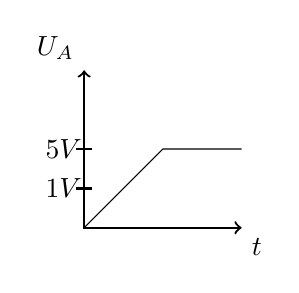
\begin{tikzpicture}
            \draw[thick,->] (-0.015,0) -- (2,0) node[anchor=north west] {$t$};
            \draw[thick,->] (0,0) -- (0,2) node[anchor=south east] {$U_{A}$};
            \draw (0,0) -- (1,1) -- (2,1);
            \draw[thick] (-0.1,1) -- (0.1,1) node[anchor=east] {$5V$};
            \draw[thick] (-0.1,0.5) -- (0.1,0.5) node[anchor=east] {$1V$};
        \end{tikzpicture}